% generated by experiments/build_paper_assets.py -- do not edit by hand
\begin{figure}[t]
\centering
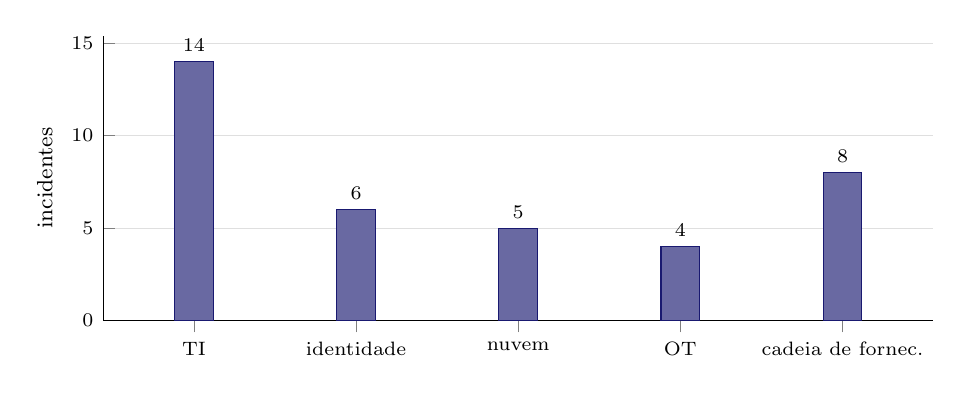
\begin{tikzpicture}
\begin{axis}[
    ybar, width=\linewidth, height=5.2cm,
    ylabel={incidentes}, symbolic x coords={TI,identidade,nuvem,OT,cadeia de fornec.},
    xtick=data, ymin=0, bar width=14pt, enlarge x limits=0.14,
    nodes near coords, nodes near coords style={font=\scriptsize},
    ticklabel style={font=\scriptsize}, label style={font=\footnotesize},
    ymajorgrids, grid style={gray!25}, axis lines*=left,
]
\addplot[fill=MidnightBlue!65, draw=MidnightBlue] coordinates {(TI,14) (identidade,6) (nuvem,5) (OT,4) (cadeia de fornec.,8)};
\end{axis}
\end{tikzpicture}
\caption{Planos atravessados pelos 20 incidentes do corpus (2017--2025). Apenas dois incidentes teriam interagido com equipamentos abaixo do nível~3 de Purdue.}
\label{fig:corpus-planes}
\end{figure}
